\chapter{Cosmology Lecture 2: From the Expanding Metric to Friedmann's Equation}

We return to the place where the previous lecture stopped. We already know how to describe an expanding universe by a scale factor \(a(t)\); what we do not yet know is what equation tells us how \(a(t)\) changes. Leonard Susskind's strategy in this lecture is very deliberate: begin with the geometry of a flat expanding coordinate grid, then step back to a simpler Newtonian problem, and only then bring the result back to cosmology. The notes below follow that order closely, with the surviving board frames kept as local witnesses to equations and sketches, following Leonard Susskind's lecture with supporting curation from LazyingArt LLC and Video2Book.

\section{From Homogeneity to the Expanding Metric}

The lecture begins by fixing the standing assumptions. Unless stated otherwise, the universe is taken to be homogeneous and isotropic. Once those assumptions are made, Hubble's law is not an accidental observational add-on; it is the kinematics forced on us by uniform expansion. At any fixed time,
\begin{equation}
v = H(t)\,d.
\end{equation}
The proportionality is linear in distance, and the crucial point is that the ``Hubble constant'' is constant only with respect to position. It is the same everywhere in space if the universe is homogeneous, but in general it changes with time.

\paragraph{Measuring rods and comoving points.}
Susskind pauses early over a natural objection: if space expands, do measuring rods expand too? The answer in the lecture is no. Bound objects do not follow the cosmological expansion in any appreciable way, because the forces holding them together are enormously stronger than the feeble effect of the background expansion on such small scales. What expands are the separations between sufficiently unbound systems such as widely separated galaxies.

This is why comoving coordinates are useful. We assign coordinates that ride with the galaxies. Then a galaxy that participates only in the smooth Hubble flow keeps the same coordinate value forever, while the physical meaning of one unit of coordinate distance changes with time. That changing conversion factor is the scale factor \(a(t)\).

For flat space the spatial metric is therefore written as
\begin{equation}
ds^2 = a(t)^2\left(dx^2+dy^2+dz^2\right).
\end{equation}
Here \(x,y,z\) are comoving coordinates. If two galaxies differ by a fixed coordinate separation \(\Delta x\) along one axis, their physical distance is
\begin{equation}
d(t)=a(t)\,\Delta x,
\end{equation}
and therefore
\begin{equation}
v=\dot d=\dot a\,\Delta x=\frac{\dot a}{a}\,d.
\end{equation}
So once the comoving metric is in place, the Hubble parameter may be read as
\begin{equation}
H(t)=\frac{\dot a}{a}.
\end{equation}

\section{Flat Spatial Slices Inside Curved Spacetime}

A flat spatial geometry does not imply flat spacetime. This is the next important turn of the lecture. If the spatial metric depends on time, then spacetime itself is curved even though each spatial slice is flat. Susskind's image is a flat rubber sheet being stretched by giants far away: the sheet remains locally flat as a sheet, but the four-dimensional spacetime story is no longer Minkowski.

Starting from the special-relativistic interval \(d\tau^2 = dt^2-ds^2\), the lecture upgrades the spatial metric to the spacetime metric
\begin{equation}
d\tau^2 = dt^2 - a(t)^2\left(dx^2+dy^2+dz^2\right).
\end{equation}
The metric coefficients do not depend on position in space; they depend only on time. That is homogeneity in metric form. In matrix language, completing the spoken description in the standard way, one writes
\begin{equation}
g_{\mu\nu}=\mathrm{diag}\!\left(1,-a(t)^2,-a(t)^2,-a(t)^2\right).
\end{equation}
The off-diagonal entries vanish. There are no \(dx\,dy\) or \(dx\,dt\) terms. It is a very simple metric, almost as simple as flat spacetime, except that the relation between spatial distance and time is itself time-dependent.

\begin{figure}
\centering

\includegraphics[width=0.58\textwidth]{lecture_02_figure_02.png}

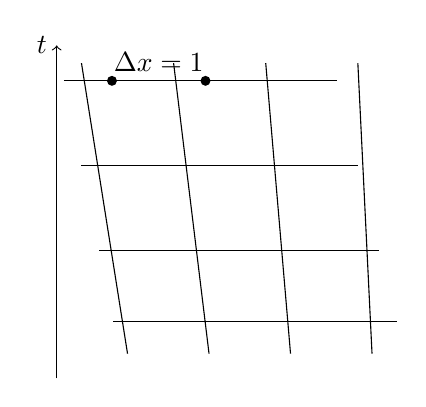
\begin{tikzpicture}[scale=0.9]
\draw[->] (0,0) -- (0,4.7) node[left]{\(t\)};
\draw (0.8,0.8) -- (4.8,0.8);
\draw (0.6,1.8) -- (4.55,1.8);
\draw (0.35,3.0) -- (4.25,3.0);
\draw (0.1,4.2) -- (3.95,4.2);

\draw (1.0,0.35) -- (0.35,4.45);
\draw (2.15,0.35) -- (1.65,4.45);
\draw (3.3,0.35) -- (2.95,4.45);
\draw (4.45,0.35) -- (4.25,4.45);

\fill (0.78,4.2) circle (2pt);
\fill (2.10,4.2) circle (2pt);
\node[above] at (1.44,4.2) {\(\Delta x = 1\)};
\end{tikzpicture}
\caption{Spacetime interval and comoving-grid sketch: the lecture frame is kept as board evidence, and the redraw below regularizes the expanding coordinate mesh that the metric describes.}
\end{figure}

The cartoon is important. At an early time one unit of coordinate separation corresponds to a small physical separation; later the same coordinate unit corresponds to a larger physical separation. Alice and Bob stay one coordinate unit apart, but the number of meters represented by that unit grows with time.

If \(a(t)\) were ever driven to zero, all physical separations would collapse to zero as well. In the lecture this is described very concretely: everything is squashed on top of everything else, and the density diverges. If \(a(t)\) grows, the universe becomes more diffuse.

\subsection{Question \& Answer}

\paragraph{Whose time is \(t\) in \(a(t)\)?}
This is the time measured by clocks moving with the galaxies. The metric is written in the comoving frame, the frame in which the distribution of galaxies is isotropic. In another frame, one moving relative to the galaxies, that simple isotropic form would not remain true.

Along the worldline of a comoving galaxy we have \(dx=dy=dz=0\), so the interval reduces to
\begin{equation}
d\tau^2 = dt^2,
\end{equation}
and therefore
\begin{equation}
dt=d\tau.
\end{equation}
So the coordinate time \(t\) is precisely the proper time measured by standard clocks carried along with the galaxies.

\section{Newtonian Warm-Up: A Projectile in a Gravitational Field}

Having set up the geometry, the lecture deliberately changes gears. Instead of deriving the dynamics from general relativity, Susskind begins with Newtonian cosmology. But even that is not his first move. Before attacking the universe, he goes back to a simpler one-body problem: a small mass \(m\) moving radially outward in the gravitational field of a heavy mass \(M\).

The point of this detour is that, for the cosmological argument he wants, energy conservation is enough. So we write down the two contributions to the energy. The kinetic term is
\begin{equation}
\frac{1}{2}mv^2,
\end{equation}
and the gravitational potential energy is
\begin{equation}
-\frac{GMm}{d}.
\end{equation}
On the board the factors are written in the order \(mMG/D\); in the cleaned formulas below we regularize this to the conventional form \(GMm/d\). The total energy is therefore
\begin{equation}
E=\frac{1}{2}mv^2-\frac{GMm}{d}.
\end{equation}
For the particular projectile under discussion, \(E\) does not depend on time.

\begin{figure}
\centering

\includegraphics[width=0.44\textwidth]{lecture_02_figure_03.png}
\hfill

\includegraphics[width=0.44\textwidth]{lecture_02_figure_04.png}

\begin{tikzpicture}[scale=1.0]
\draw (0,0) circle (0.42);
\draw (0,0) circle (0.28);
\draw (0,0) circle (0.14);
\node at (0,-0.8) {\(M\)};

\fill (1.25,0) circle (2pt);
\node[below] at (1.25,0) {\(m\)};
\draw[->] (1.35,0) -- (3.0,0);

\node at (5.0,0.4) {\(\frac{1}{2}mv^2\)};
\node at (7.4,0.4) {\(-\)};
\node at (9.1,0.4) {\(\frac{GMm}{d}\)};
\end{tikzpicture}
\caption{Newtonian warm-up on the board. The first frame isolates the kinetic term; the second adds the negative gravitational potential. The redraw regularizes the source--test-mass setup without replacing the original board evidence.}
\end{figure}

\subsection{Question \& Answer}

\paragraph{Why is the gravitational potential energy negative?}
The lecture answers this with a picture rather than an abstract sign convention. Forget the constants for a moment and look at \(1/D\). It decreases as \(D\) grows. Then \(-1/D\) is the same curve upside down. Forces push toward decreasing potential energy. For gravity that means toward smaller radius. An attractive force therefore corresponds to a potential that becomes more negative as the distance decreases.

\begin{equation}
V(d)\propto -\frac{1}{d}.
\end{equation}

\begin{figure}
\centering

\includegraphics[width=0.46\textwidth]{lecture_02_figure_05.png}

\begin{tikzpicture}[scale=1.0]
\draw[->] (0,0) -- (4.6,0) node[right]{\(D\)};
\draw[->] (0,-2.2) -- (0,2.2);

\draw[domain=0.35:4.0,smooth,variable=\x] plot (\x,{1/\x});
\draw[domain=0.35:4.0,smooth,variable=\x] plot (\x,{-1/\x});

\node at (3.35,0.95) {\(\frac{1}{D}\)};
\node at (3.35,-1.0) {\(-\frac{1}{D}\)};
\end{tikzpicture}
\caption{Qualitative plots of \(1/D\) and \(-1/D\). The lecture uses the inverted curve to explain why an attractive force points toward decreasing potential energy.}
\end{figure}

With that sign understood, the warm-up problem is complete: the projectile carries a conserved energy \(E\), and the sign of \(E\) tells us what kind of motion is possible.

\section{Escape Velocity and the Three Energy Regimes}

Now the lecture turns from formula to behavior. There are only three possibilities:

\begin{itemize}
\item If \(E<0\), the projectile is bound. It rises, slows, reaches a maximum distance, and falls back.
\item If \(E=0\), the projectile has exactly the escape velocity. The distance keeps increasing forever, but the speed decreases toward zero.
\item If \(E>0\), the projectile escapes completely. Gravity produces some deceleration at first, but not enough to prevent the particle from moving off with a nonzero asymptotic speed.
\end{itemize}

This is the moment when the local Newtonian problem becomes a cosmological analogy. Replace the Earth and the projectile by a homogeneous expanding distribution of galaxies. Then the same three qualitative futures are available: enough initial recession to escape forever, too little recession and a later re-collapse, or the critical case that sits exactly on the boundary between the two.

For very small initial outward speed, the lecture emphasizes that the negative potential term dominates:
\begin{figure}
\centering

\includegraphics[width=0.62\textwidth]{lecture_02_figure_06.png}
\caption{Later emphasis frame: for sufficiently small outward speed, the negative potential term dominates the total energy.}
\end{figure}

In the cosmological language, this is the content of the escape-velocity analogy. The universe can be above escape velocity, below escape velocity, or exactly at escape velocity.

\section{Newton's Shell Theorem and the Cosmological Reduction}

The next step is the conceptual hinge of the lecture. We want to use the same energy equation for a galaxy in a homogeneous universe, but then which masses should count in the force? Newton's shell theorem gives the answer.

For a spherically symmetric mass distribution, the force on a particle at radius \(d\) is exactly the same as if all the mass inside radius \(d\) were concentrated at the center, while all mass outside radius \(d\) contributes no net force. The theorem is special to the inverse-square law, and Susskind dwells on that surprise for a while, because it is what makes the cosmological reduction possible at all.

Now choose any galaxy and, in our temporary egotistical imagination, call it the center. Because the universe is homogeneous and isotropic, no physical result can depend on which galaxy we chose. Pick a second galaxy at comoving coordinate \(x\). Draw a sphere centered on the first galaxy and passing through the second. Then only the mass inside that sphere matters for the motion of the second galaxy.

Two points matter here.

First, the choice of center is arbitrary. Anybody may place himself at the center, and the same equation must come out.

Second, the sphere expands with the galaxies. It therefore encloses the same galaxies for all time, and hence the same total mass for that comoving sphere. This is exactly what makes a conserved-energy treatment sensible.

\section{From Galaxy Energetics to Friedmann's Equation}

We now write the Newtonian energy equation in a form suited to cosmology. After dividing by the test mass, we may write
\begin{equation}
\frac{v^2}{2}-\frac{GM(d)}{d}=\varepsilon(x),
\end{equation}
where \(\varepsilon(x)\) is constant in time for the galaxy at coordinate \(x\). It need not be the same for different galaxies.

The physical distance to that galaxy is
\begin{equation}
d=a(t)x,
\end{equation}
and because \(x\) is comoving,
\begin{equation}
v=\dot d=\dot a\,x.
\end{equation}
If the density is \(\rho(t)\), then the mass enclosed by the sphere of radius \(d\) is
\begin{equation}
M(d)=\frac{4\pi}{3}\rho\,d^3=\frac{4\pi}{3}\rho\,a^3x^3.
\end{equation}
Substituting into the energy equation gives
\begin{align}
\frac{(\dot a x)^2}{2}-\frac{G\left(\frac{4\pi}{3}\rho\,a^3x^3\right)}{ax} &= \varepsilon(x), \\
\frac{\dot a^2x^2}{2}-\frac{4\pi G}{3}\rho\,a^2x^2 &= \varepsilon(x).
\end{align}

This is the place where the lecture slows down and insists on the role of the \(x^2\). The whole left-hand side is proportional to \(x^2\), and everything except \(x\) is the same for every galaxy. Therefore the right-hand side must also be proportional to \(x^2\). The word ``constant'' meant constant in time for a given galaxy, not universal across all galaxies. Consistency forces
\begin{equation}
\varepsilon(x)=-\frac{k}{2}\,x^2,
\end{equation}
where the normalization of \(k\) is conventional. Dividing through by \(x^2/2\) yields
\begin{equation}
\dot a^2=\frac{8\pi G}{3}\rho\,a^2-k.
\end{equation}
Dividing once more by \(a^2\), we arrive at the historical form emphasized in the lecture,
\begin{equation}
\left(\frac{\dot a}{a}\right)^2=\frac{8\pi G}{3}\rho-\frac{k}{a^2}.
\end{equation}

This is Friedmann's equation as obtained from Newtonian reasoning. The lecture is careful not to oversell the derivation: it is a model, and the full geometric interpretation belongs to general relativity. But the structure is already suggestive. The left-hand side involves the metric through \(a(t)\), while the right-hand side involves the density of matter.

In units with \(c=1\), \(k\) is dimensionless. Its sign may be positive, negative, or zero. The critical case \(k=0\) is the analog of exact escape velocity.

\section{Matter Density, the Critical Case, and the Age of the Universe}

To solve Friedmann's equation we still need the time dependence of \(\rho\). Susskind introduces it by choosing a unit comoving cube. Let the mass inside that cube be \(m_{\Box}\). The lecture reuses the letter \(m\) here, but it is clearer to distinguish this mass from the earlier test particle.

The physical side length of a unit comoving cube is \(a(t)\), so its physical volume is \(a(t)^3\). Therefore
\begin{equation}
\rho(t)=\frac{m_{\Box}}{a(t)^3}.
\end{equation}
In the critical case \(k=0\), Friedmann's equation becomes
\begin{equation}
\left(\frac{\dot a}{a}\right)^2=\frac{8\pi G\,m_{\Box}}{3a^3}.
\end{equation}

Now comes the worked solution. The lecture solves this by guessing a power law,
\begin{equation}
a(t)=ct^p,
\end{equation}
with constants \(c\) and \(p\) to be determined. Then
\begin{equation}
\dot a = cp\,t^{p-1},
\end{equation}
so that
\begin{equation}
\frac{\dot a}{a}=\frac{p}{t}.
\end{equation}
Substituting into the equation gives
\begin{equation}
\frac{p^2}{t^2}=\frac{8\pi G\,m_{\Box}}{3c^3\,t^{3p}}.
\end{equation}
For this to hold for all \(t\), the powers of \(t\) must match:
\begin{equation}
3p=2,
\end{equation}
hence
\begin{equation}
p=\frac{2}{3}.
\end{equation}
Then the coefficients must match as well:
\begin{equation}
\frac{4}{9}=\frac{8\pi G\,m_{\Box}}{3c^3},
\end{equation}
and therefore
\begin{equation}
c^3=6\pi G\,m_{\Box}.
\end{equation}
So the critical matter-dominated solution is
\begin{equation}
a(t)=\left(6\pi G\,m_{\Box}\right)^{1/3}t^{2/3}.
\end{equation}
More generally one may write
\begin{equation}
a(t)\propto (t-t_0)^{2/3},
\end{equation}
and absorb the remaining integration constant into a choice of the origin of time. If we choose \(t=0\) to mean the moment when \(a=0\), the solution takes the simpler form above.

The lecture is careful here. To say \(a=0\) literally is to push the model past where Newtonian reasoning should be trusted. But the physical meaning is clear enough: at sufficiently early time the universe was extraordinarily dense, with all scales driven down toward zero. This is the Big Bang limit of the model.

The Hubble parameter is now explicit:
\begin{equation}
H(t)=\frac{\dot a}{a}=\frac{2}{3t}.
\end{equation}
So in this model the age of the universe is
\begin{equation}
t=\frac{2}{3H}.
\end{equation}
This is one of the lecture's main payoffs. The Hubble ``constant'' is not constant in time at all; it falls like \(1/t\). But if we measure it today, then in the \(k=0\), matter-dominated model we may infer the age of the universe. In the lecture Susskind quotes an age of roughly \(13\) to \(14\) billion years and remarks that \(k=0\) is, observationally, a very realistic approximation.

\subsection{Question \& Answer}

\paragraph{Why does the age estimate not depend on the arbitrary fiducial box mass?}
The subtle point is that the fiducial box is conventional. If we double the side length of the chosen comoving box, the mass inside it increases by a factor of \(8\), while the quantity \(m_{\Box}^{1/3}\) increases by a factor of \(2\). At the same time the corresponding normalization of \(a\) changes by the same factor. What is physical is the density
\begin{equation}
\rho=\frac{m_{\Box}}{a^3},
\end{equation}
not \(a\) or \(m_{\Box}\) separately.

In the explicit solution the dependence on \(m_{\Box}\) sits entirely in the constant \(c\). But
\begin{equation}
a(t)=ct^{2/3}
\end{equation}
implies
\begin{equation}
\dot a = \frac{2}{3}c\,t^{-1/3},
\end{equation}
and therefore
\begin{equation}
\frac{\dot a}{a}=\frac{\frac{2}{3}c\,t^{-1/3}}{ct^{2/3}}=\frac{2}{3t}.
\end{equation}
The constant \(c\) cancels. That is why the age relation \(t=2/(3H)\) does not depend on the arbitrary normalization of the fiducial box in the critical model.

This is also the right place to hear the final conceptual reinterpretation foreshadowed at the end of the lecture. Rearranged as
\begin{equation}
\frac{\dot a^2}{a^2}-\frac{k}{a^2}=\frac{8\pi G}{3}\rho,
\end{equation}
the left-hand side is geometric, built from the scale factor and, in the next lecture, from spatial curvature. The right-hand side is matter density, or in relativistic language energy density. That is exactly the sort of relation Einstein's equations are supposed to produce.

\section{Summary}

The lecture moves in a very clean arc. Homogeneity and isotropy give the kinematics of expansion, the comoving metric makes the scale factor precise, a Newtonian escape-velocity problem supplies the right dynamical intuition, and Newton's shell theorem reduces the many-body universe to an effective one-body problem. From there one obtains Friedmann's equation,
\begin{equation}
\left(\frac{\dot a}{a}\right)^2=\frac{8\pi G}{3}\rho-\frac{k}{a^2},
\end{equation}
and in the critical matter-dominated case,
\begin{equation}
a(t)\propto t^{2/3}, \qquad H(t)=\frac{2}{3t}.
\end{equation}
That already gives a usable age estimate and, just as important, it sets up the next lecture's deeper interpretation: geometry on the left, energy density on the right, and curvature waiting to be brought fully into view.